%% Supplementary material for the CBM submission. Build: latexmk -pdf supplementary.tex
\documentclass[11pt]{article}
\usepackage[T1]{fontenc}
\usepackage{lmodern}
\usepackage[margin=2.2cm]{geometry}
\usepackage{amsmath,amssymb}
\usepackage{booktabs,tabularx,array,longtable}
\usepackage{graphicx,xcolor}
\usepackage{pdflscape}
\usepackage{tikz}
\usetikzlibrary{arrows.meta,positioning,fit,backgrounds}
\usepackage[hidelinks]{hyperref}
\usepackage{xurl}
\usepackage[font=small,labelfont=bf]{caption}
\renewcommand{\thefigure}{S\arabic{figure}}
\renewcommand{\thetable}{S\arabic{table}}
\renewcommand{\thesection}{S\arabic{section}}
\renewcommand{\theequation}{S\arabic{equation}}
\newcolumntype{L}{>{\raggedright\arraybackslash}X}
\definecolor{ink2}{HTML}{52514E}
\definecolor{edge}{HTML}{898781}
\definecolor{accent}{HTML}{2A78D6}
\definecolor{tint}{HTML}{F0EFEC}

\title{Supplementary material for\\[4pt]\large ``Leakage-controlled stacking and recursive feature elimination for type~2 diabetes prediction: a rigorous evaluation on the PIMA dataset''}
\author{Subrahmanyam Tanala}
\date{}

\begin{document}
\maketitle

\section{Validation design: where each loop runs}

Figure~\ref{fig:nested} shows the complete validation design. There are three nested levels. The \emph{outer} level is the 5$\times$10-fold repeated cross-validation used for model comparison. Within each outer training part there are two \emph{inner} levels: the 5-fold cross-validation that RFECV uses to choose the subset size, and the 5-fold split that produces out-of-fold probabilities for the stacking meta-learner. The 154-patient hold-out set is separated before any modelling and is used once, by the final pipeline refitted on all 614 development patients.

\begin{figure}[!htbp]
\centering
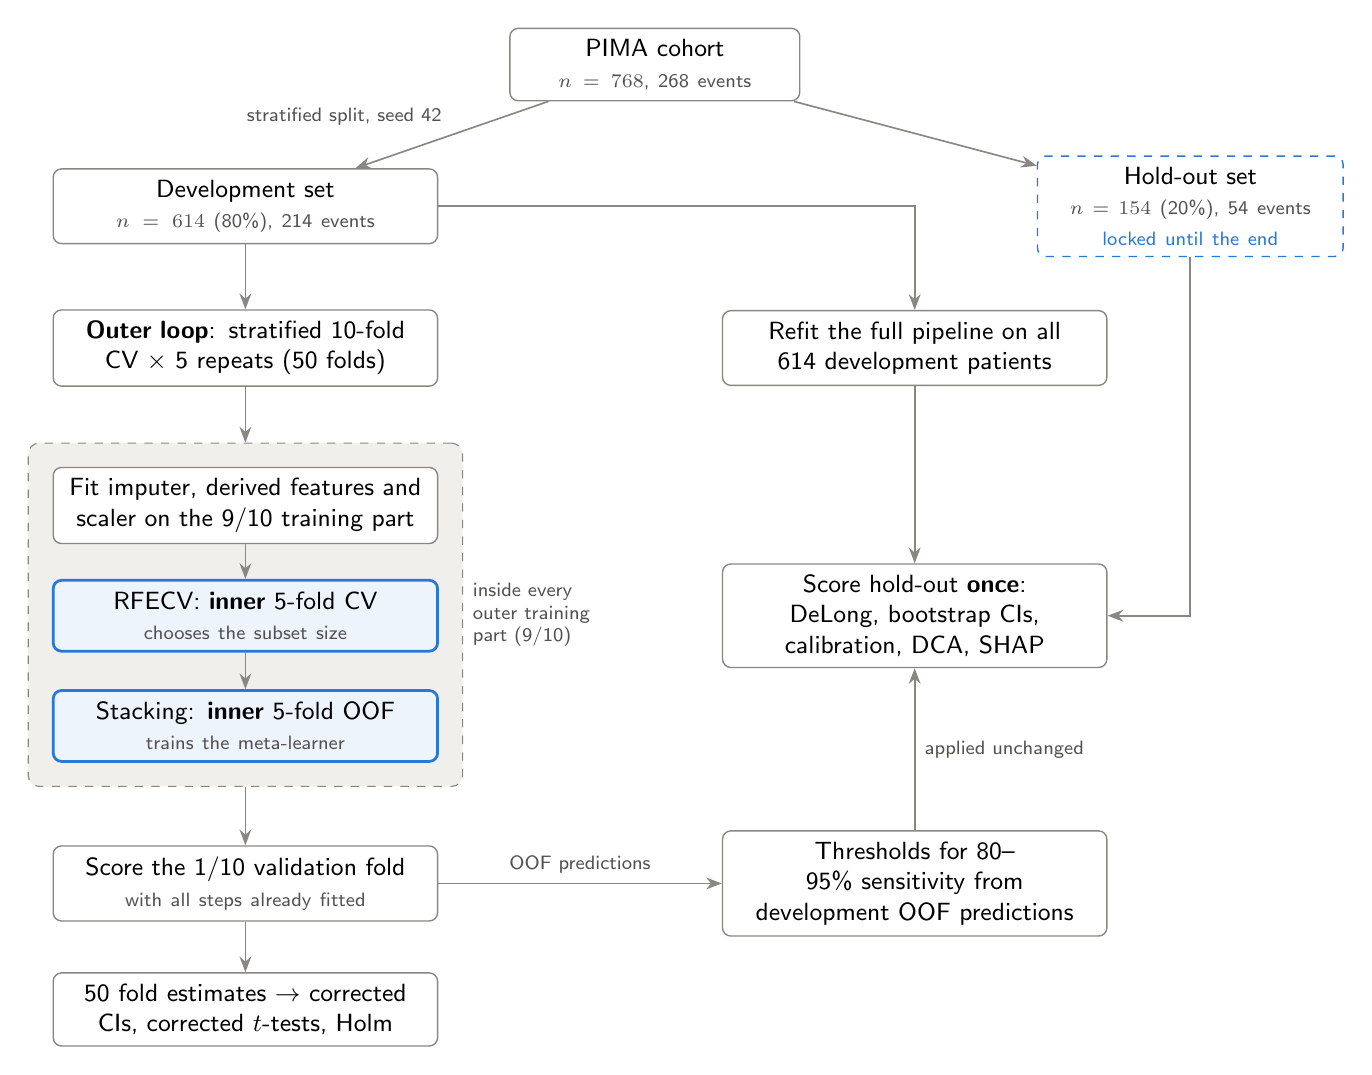
\begin{tikzpicture}[
  font=\sffamily\small, >={Stealth[length=2mm]},
  every node/.append style={execute at begin node={\hyphenpenalty=10000\relax}},
  box/.style={draw=edge, rounded corners=3pt, align=center, minimum height=9mm, inner sep=4pt, line width=0.5pt, fill=white, text width=46mm},
  key/.style={box, draw=accent, line width=1pt, fill=accent!8},
  note/.style={font=\sffamily\scriptsize, text=ink2, align=center},
  arr/.style={->, draw=edge, line width=0.6pt}]
\node[box, text width=34mm] (data) at (5.2,0) {PIMA cohort\\{\scriptsize\color{ink2} $n=768$, 268 events}};
\node[box] (dev) at (0,-1.8) {Development set\\{\scriptsize\color{ink2} $n=614$ (80\%), 214 events}};
\node[box, draw=accent, dashed, text width=36mm] (hold) at (12,-1.8) {Hold-out set\\{\scriptsize\color{ink2} $n=154$ (20\%), 54 events}\\{\scriptsize\color{accent} locked until the end}};
\draw[arr] (data) -- node[note, above left] {stratified split, seed 42} (dev);
\draw[arr] (data) -- (hold);
\node[box] (outer) at (0,-3.6) {\textbf{Outer loop}: stratified 10-fold\\CV $\times$ 5 repeats (50 folds)};
\draw[arr] (dev) -- (outer);
\node[box] (prep) at (0,-5.6) {Fit imputer, derived features and scaler on the 9/10 training part};
\node[key] (rfe) at (0,-7.0) {RFECV: \textbf{inner} 5-fold CV\\{\scriptsize\color{ink2} chooses the subset size}};
\node[key] (stk) at (0,-8.4) {Stacking: \textbf{inner} 5-fold OOF\\{\scriptsize\color{ink2} trains the meta-learner}};
\begin{scope}[on background layer]
\node[draw=edge, dashed, rounded corners=4pt, fill=tint, inner sep=3mm, fit=(prep)(rfe)(stk), label={[note, anchor=west, align=left]east:inside every\\outer training\\part (9/10)}] (inner) {};
\end{scope}
\draw[arr] (outer) -- (inner);
\draw[arr] (prep) -- (rfe); \draw[arr] (rfe) -- (stk);
\node[box] (score) at (0,-10.4) {Score the 1/10 validation fold\\{\scriptsize\color{ink2} with all steps already fitted}};
\draw[arr] (inner) -- (score);
\node[box] (agg) at (0,-12.0) {50 fold estimates $\to$ corrected CIs, corrected $t$-tests, Holm};
\draw[arr] (score) -- (agg);
\node[box] (refit) at (8.5,-3.6) {Refit the full pipeline on all 614 development patients};
\draw[arr] (dev.east) -| (refit.north);
\node[box] (eval) at (8.5,-7.0) {Score hold-out \textbf{once}: DeLong, bootstrap CIs, calibration, DCA, SHAP};
\draw[arr] (refit) -- (eval);
\draw[arr] (hold.south) |- (eval.east);
\node[box] (thr) at (8.5,-10.4) {Thresholds for 80--95\% sensitivity from development OOF predictions};
\draw[arr] (score) -- node[note, above] {OOF predictions} (thr);
\draw[arr] (thr) -- node[note, right] {applied unchanged} (eval);
\end{tikzpicture}
\caption{Nested validation design. Blue boxes mark the two inner resampling loops that run inside every outer training part. Nothing from an outer validation fold or from the hold-out set is used to fit any step.}
\label{fig:nested}
\end{figure}

\section{Statistical testing procedure}

\paragraph{Repeated cross-validation}
Let $x_{rk}$ be the value of a metric on fold $k$ of repeat $r$ ($r=1,\dots,5$; $k=1,\dots,10$; $J=50$). The point estimate is $\bar x = J^{-1}\sum_{r,k} x_{rk}$. Fold estimates share most of their training data, so the naive variance $s^2/J$ is too small. Following Nadeau and Bengio, we use
\begin{equation}
\widehat{\operatorname{Var}}(\bar x) = \left(\frac{1}{J} + \frac{n_{\mathrm{test}}}{n_{\mathrm{train}}}\right) s^2, \qquad \frac{n_{\mathrm{test}}}{n_{\mathrm{train}}} = \frac{1}{9},
\end{equation}
with $s^2$ the sample variance of the $J$ fold estimates. 95\% confidence intervals are $\bar x \pm t_{0.975,\,J-1}\sqrt{\widehat{\operatorname{Var}}}$.

\paragraph{Paired comparisons}
For a configuration $A$ and the reference $B$ (logistic regression on all features), $d_{rk} = x^{A}_{rk} - x^{B}_{rk}$ is computed on identical folds. The corrected resampled statistic is $t = \bar d / \sqrt{(1/J + 1/9)\,s_d^2}$, referred to a $t$ distribution with $J-1 = 49$ degrees of freedom (two-sided). The 22 $p$-values (11 learners $\times$ 2 feature sets, plus LR-ranked RFECV, minus the reference) are adjusted with the Holm step-down procedure.

\paragraph{Why this test}
The corrected resampled $t$-test is designed for exactly this setting, where fold estimates from repeated $k$-fold cross-validation are correlated. In simulation studies it keeps the type~I error close to the nominal level and replicates well across random partitions, whereas the uncorrected paired $t$-test is anti-conservative. Alternatives such as a nested bootstrap of the whole pipeline or Bayesian correlated $t$-tests are valid. However, a nested bootstrap would have required thousands of refits of RFECV and the stack (about 45~s each), and the conclusions here are far from any decision boundary: the stacking--logistic-regression difference is $+0.001$ with an adjusted $p = 1.00$.

\paragraph{Hold-out set}
ROC-AUC confidence intervals and pairwise comparisons on the 154 hold-out patients use DeLong's non-parametric covariance (fast mid-rank implementation), with Holm adjustment over six comparisons against stacking + RFECV. All other metrics use 95\% percentile bootstrap intervals from 2000 resamples of hold-out patients; resamples containing a single class are discarded.

\paragraph{Calibration and thresholds}
The calibration intercept is estimated from $\operatorname{logit} P(y=1) = a + \operatorname{logit}\hat p$ (offset model) and the slope from $\operatorname{logit} P(y=1) = a' + b\operatorname{logit}\hat p$, both by Newton--Raphson maximum likelihood. For a target sensitivity $s$, the threshold is the largest value $t$ for which at least $\lceil s\,n_+\rceil$ of the $n_+$ development-set positives have an out-of-fold probability (averaged over the five repeats) of at least $t$.

\section{Full cross-validated results}

\begin{landscape}
\begin{table}[p]
\centering
\caption{All 23 configurations from 5$\times$10-fold repeated cross-validation on the development set ($n=614$). Means with Nadeau--Bengio corrected 95\% CIs beneath. ``+ RFECV'' is the common random-forest-ranked RFECV subset. The last two columns give the unadjusted and Holm-adjusted corrected resampled $t$-test $p$-values for the ROC-AUC difference from logistic regression on all features. Threshold-based metrics use 0.5.}
\label{tab:s-cv}
\scriptsize
\setlength{\tabcolsep}{3pt}
\begin{tabular}{lrcccccccccrr}
\toprule
Model & Feat. & Acc. & Bal.\ acc. & Prec. & Sens. & Spec. & F1 & MCC & ROC-AUC & Brier & $p$ & $p_{\mathrm{Holm}}$ \\
\midrule
Stacking & 16.0 & 0.759 & 0.760 & 0.635 & 0.763 & 0.757 & 0.689 & 0.505 & 0.846 & 0.164 & 0.586 & 1.000 \\
 &  & {\scriptsize\color{gray}(0.719--0.799)} & {\scriptsize\color{gray}(0.722--0.797)} & {\scriptsize\color{gray}(0.579--0.691)} & {\scriptsize\color{gray}(0.710--0.815)} & {\scriptsize\color{gray}(0.700--0.814)} & {\scriptsize\color{gray}(0.646--0.732)} & {\scriptsize\color{gray}(0.431--0.580)} & {\scriptsize\color{gray}(0.812--0.880)} & {\scriptsize\color{gray}(0.144--0.183)} &  &  \\[2pt]
Stacking + RFECV & 12.0 & 0.756 & 0.755 & 0.631 & 0.753 & 0.757 & 0.684 & 0.497 & 0.843 & 0.165 & 0.890 & 1.000 \\
 &  & {\scriptsize\color{gray}(0.714--0.797)} & {\scriptsize\color{gray}(0.715--0.795)} & {\scriptsize\color{gray}(0.574--0.688)} & {\scriptsize\color{gray}(0.697--0.810)} & {\scriptsize\color{gray}(0.700--0.814)} & {\scriptsize\color{gray}(0.638--0.730)} & {\scriptsize\color{gray}(0.418--0.575)} & {\scriptsize\color{gray}(0.809--0.878)} & {\scriptsize\color{gray}(0.144--0.185)} &  &  \\[2pt]
Logistic regression & 16.0 & 0.764 & 0.759 & 0.646 & 0.744 & 0.775 & 0.688 & 0.507 & 0.842 & 0.163 & -- & -- \\
 &  & {\scriptsize\color{gray}(0.727--0.801)} & {\scriptsize\color{gray}(0.725--0.794)} & {\scriptsize\color{gray}(0.592--0.700)} & {\scriptsize\color{gray}(0.690--0.798)} & {\scriptsize\color{gray}(0.721--0.828)} & {\scriptsize\color{gray}(0.647--0.729)} & {\scriptsize\color{gray}(0.438--0.576)} & {\scriptsize\color{gray}(0.809--0.875)} & {\scriptsize\color{gray}(0.144--0.183)} &  &  \\[2pt]
Logistic regression + RFECV & 12.0 & 0.760 & 0.750 & 0.647 & 0.717 & 0.782 & 0.676 & 0.492 & 0.842 & 0.163 & 0.997 & 1.000 \\
 &  & {\scriptsize\color{gray}(0.721--0.798)} & {\scriptsize\color{gray}(0.713--0.786)} & {\scriptsize\color{gray}(0.588--0.706)} & {\scriptsize\color{gray}(0.664--0.770)} & {\scriptsize\color{gray}(0.727--0.838)} & {\scriptsize\color{gray}(0.633--0.720)} & {\scriptsize\color{gray}(0.418--0.566)} & {\scriptsize\color{gray}(0.811--0.873)} & {\scriptsize\color{gray}(0.145--0.182)} &  &  \\[2pt]
LR (LR-ranked RFECV) & 10.1 & 0.760 & 0.754 & 0.641 & 0.731 & 0.776 & 0.680 & 0.496 & 0.840 & 0.164 & 0.487 & 1.000 \\
 &  & {\scriptsize\color{gray}(0.725--0.796)} & {\scriptsize\color{gray}(0.717--0.790)} & {\scriptsize\color{gray}(0.591--0.692)} & {\scriptsize\color{gray}(0.671--0.791)} & {\scriptsize\color{gray}(0.728--0.824)} & {\scriptsize\color{gray}(0.637--0.724)} & {\scriptsize\color{gray}(0.426--0.567)} & {\scriptsize\color{gray}(0.808--0.873)} & {\scriptsize\color{gray}(0.145--0.183)} &  &  \\[2pt]
SVM & 16.0 & 0.775 & 0.747 & 0.695 & 0.655 & 0.840 & 0.670 & 0.505 & 0.840 & 0.156 & 0.796 & 1.000 \\
 &  & {\scriptsize\color{gray}(0.735--0.815)} & {\scriptsize\color{gray}(0.705--0.790)} & {\scriptsize\color{gray}(0.624--0.767)} & {\scriptsize\color{gray}(0.587--0.723)} & {\scriptsize\color{gray}(0.790--0.889)} & {\scriptsize\color{gray}(0.614--0.726)} & {\scriptsize\color{gray}(0.418--0.591)} & {\scriptsize\color{gray}(0.802--0.878)} & {\scriptsize\color{gray}(0.138--0.175)} &  &  \\[2pt]
SVM + RFECV & 12.0 & 0.765 & 0.736 & 0.680 & 0.643 & 0.830 & 0.656 & 0.483 & 0.837 & 0.158 & 0.577 & 1.000 \\
 &  & {\scriptsize\color{gray}(0.722--0.808)} & {\scriptsize\color{gray}(0.693--0.780)} & {\scriptsize\color{gray}(0.605--0.755)} & {\scriptsize\color{gray}(0.578--0.708)} & {\scriptsize\color{gray}(0.776--0.884)} & {\scriptsize\color{gray}(0.599--0.713)} & {\scriptsize\color{gray}(0.393--0.572)} & {\scriptsize\color{gray}(0.800--0.873)} & {\scriptsize\color{gray}(0.140--0.176)} &  &  \\[2pt]
Extra trees + RFECV & 12.0 & 0.753 & 0.739 & 0.642 & 0.693 & 0.786 & 0.662 & 0.474 & 0.835 & 0.161 & 0.429 & 1.000 \\
 &  & {\scriptsize\color{gray}(0.713--0.794)} & {\scriptsize\color{gray}(0.698--0.780)} & {\scriptsize\color{gray}(0.581--0.703)} & {\scriptsize\color{gray}(0.627--0.759)} & {\scriptsize\color{gray}(0.732--0.840)} & {\scriptsize\color{gray}(0.612--0.712)} & {\scriptsize\color{gray}(0.393--0.556)} & {\scriptsize\color{gray}(0.798--0.872)} & {\scriptsize\color{gray}(0.142--0.179)} &  &  \\[2pt]
Extra trees & 16.0 & 0.753 & 0.735 & 0.647 & 0.676 & 0.794 & 0.656 & 0.469 & 0.835 & 0.160 & 0.448 & 1.000 \\
 &  & {\scriptsize\color{gray}(0.707--0.798)} & {\scriptsize\color{gray}(0.690--0.780)} & {\scriptsize\color{gray}(0.576--0.717)} & {\scriptsize\color{gray}(0.609--0.743)} & {\scriptsize\color{gray}(0.736--0.852)} & {\scriptsize\color{gray}(0.601--0.712)} & {\scriptsize\color{gray}(0.377--0.560)} & {\scriptsize\color{gray}(0.795--0.874)} & {\scriptsize\color{gray}(0.140--0.181)} &  &  \\[2pt]
Naive Bayes + RFECV & 12.0 & 0.762 & 0.730 & 0.682 & 0.624 & 0.836 & 0.646 & 0.473 & 0.832 & 0.205 & 0.263 & 1.000 \\
 &  & {\scriptsize\color{gray}(0.725--0.799)} & {\scriptsize\color{gray}(0.692--0.768)} & {\scriptsize\color{gray}(0.607--0.756)} & {\scriptsize\color{gray}(0.564--0.683)} & {\scriptsize\color{gray}(0.787--0.886)} & {\scriptsize\color{gray}(0.595--0.698)} & {\scriptsize\color{gray}(0.393--0.554)} & {\scriptsize\color{gray}(0.797--0.867)} & {\scriptsize\color{gray}(0.174--0.235)} &  &  \\[2pt]
Random forest & 16.0 & 0.756 & 0.746 & 0.641 & 0.712 & 0.780 & 0.671 & 0.484 & 0.831 & 0.164 & 0.269 & 1.000 \\
 &  & {\scriptsize\color{gray}(0.710--0.802)} & {\scriptsize\color{gray}(0.698--0.793)} & {\scriptsize\color{gray}(0.575--0.707)} & {\scriptsize\color{gray}(0.639--0.785)} & {\scriptsize\color{gray}(0.724--0.836)} & {\scriptsize\color{gray}(0.613--0.728)} & {\scriptsize\color{gray}(0.390--0.578)} & {\scriptsize\color{gray}(0.795--0.868)} & {\scriptsize\color{gray}(0.144--0.184)} &  &  \\[2pt]
Random forest + RFECV & 12.0 & 0.759 & 0.750 & 0.645 & 0.718 & 0.781 & 0.676 & 0.492 & 0.831 & 0.164 & 0.262 & 1.000 \\
 &  & {\scriptsize\color{gray}(0.715--0.804)} & {\scriptsize\color{gray}(0.705--0.794)} & {\scriptsize\color{gray}(0.580--0.711)} & {\scriptsize\color{gray}(0.652--0.785)} & {\scriptsize\color{gray}(0.725--0.838)} & {\scriptsize\color{gray}(0.622--0.730)} & {\scriptsize\color{gray}(0.403--0.581)} & {\scriptsize\color{gray}(0.797--0.866)} & {\scriptsize\color{gray}(0.145--0.184)} &  &  \\[2pt]
Gradient boosting & 16.0 & 0.746 & 0.711 & 0.657 & 0.595 & 0.828 & 0.618 & 0.436 & 0.831 & 0.164 & 0.294 & 1.000 \\
 &  & {\scriptsize\color{gray}(0.709--0.784)} & {\scriptsize\color{gray}(0.670--0.752)} & {\scriptsize\color{gray}(0.589--0.726)} & {\scriptsize\color{gray}(0.520--0.669)} & {\scriptsize\color{gray}(0.779--0.876)} & {\scriptsize\color{gray}(0.562--0.675)} & {\scriptsize\color{gray}(0.353--0.518)} & {\scriptsize\color{gray}(0.798--0.863)} & {\scriptsize\color{gray}(0.145--0.183)} &  &  \\[2pt]
Naive Bayes & 16.0 & 0.773 & 0.739 & 0.701 & 0.626 & 0.852 & 0.657 & 0.494 & 0.830 & 0.205 & 0.159 & 1.000 \\
 &  & {\scriptsize\color{gray}(0.739--0.807)} & {\scriptsize\color{gray}(0.703--0.775)} & {\scriptsize\color{gray}(0.636--0.766)} & {\scriptsize\color{gray}(0.566--0.686)} & {\scriptsize\color{gray}(0.808--0.895)} & {\scriptsize\color{gray}(0.608--0.706)} & {\scriptsize\color{gray}(0.420--0.568)} & {\scriptsize\color{gray}(0.793--0.867)} & {\scriptsize\color{gray}(0.175--0.235)} &  &  \\[2pt]
Gradient boosting + RFECV & 12.0 & 0.748 & 0.714 & 0.660 & 0.601 & 0.827 & 0.623 & 0.441 & 0.830 & 0.164 & 0.291 & 1.000 \\
 &  & {\scriptsize\color{gray}(0.709--0.788)} & {\scriptsize\color{gray}(0.671--0.757)} & {\scriptsize\color{gray}(0.588--0.733)} & {\scriptsize\color{gray}(0.525--0.677)} & {\scriptsize\color{gray}(0.776--0.878)} & {\scriptsize\color{gray}(0.564--0.682)} & {\scriptsize\color{gray}(0.354--0.528)} & {\scriptsize\color{gray}(0.798--0.862)} & {\scriptsize\color{gray}(0.145--0.183)} &  &  \\[2pt]
KNN & 16.0 & 0.760 & 0.726 & 0.681 & 0.611 & 0.841 & 0.639 & 0.466 & 0.824 & 0.162 & 0.108 & 1.000 \\
 &  & {\scriptsize\color{gray}(0.718--0.802)} & {\scriptsize\color{gray}(0.681--0.770)} & {\scriptsize\color{gray}(0.605--0.757)} & {\scriptsize\color{gray}(0.541--0.680)} & {\scriptsize\color{gray}(0.790--0.891)} & {\scriptsize\color{gray}(0.578--0.700)} & {\scriptsize\color{gray}(0.375--0.558)} & {\scriptsize\color{gray}(0.781--0.866)} & {\scriptsize\color{gray}(0.141--0.183)} &  &  \\[2pt]
XGBoost & 16.0 & 0.744 & 0.713 & 0.650 & 0.611 & 0.816 & 0.625 & 0.436 & 0.821 & 0.173 & 0.056 & 0.954 \\
 &  & {\scriptsize\color{gray}(0.701--0.787)} & {\scriptsize\color{gray}(0.670--0.757)} & {\scriptsize\color{gray}(0.576--0.723)} & {\scriptsize\color{gray}(0.543--0.678)} & {\scriptsize\color{gray}(0.761--0.871)} & {\scriptsize\color{gray}(0.567--0.683)} & {\scriptsize\color{gray}(0.346--0.527)} & {\scriptsize\color{gray}(0.784--0.857)} & {\scriptsize\color{gray}(0.149--0.196)} &  &  \\[2pt]
KNN + RFECV & 12.0 & 0.757 & 0.721 & 0.675 & 0.604 & 0.839 & 0.632 & 0.458 & 0.821 & 0.163 & 0.110 & 1.000 \\
 &  & {\scriptsize\color{gray}(0.713--0.800)} & {\scriptsize\color{gray}(0.674--0.769)} & {\scriptsize\color{gray}(0.600--0.750)} & {\scriptsize\color{gray}(0.525--0.683)} & {\scriptsize\color{gray}(0.788--0.889)} & {\scriptsize\color{gray}(0.567--0.697)} & {\scriptsize\color{gray}(0.361--0.554)} & {\scriptsize\color{gray}(0.777--0.865)} & {\scriptsize\color{gray}(0.143--0.183)} &  &  \\[2pt]
XGBoost + RFECV & 12.0 & 0.746 & 0.716 & 0.651 & 0.615 & 0.817 & 0.627 & 0.440 & 0.820 & 0.172 & 0.033 & 0.586 \\
 &  & {\scriptsize\color{gray}(0.707--0.785)} & {\scriptsize\color{gray}(0.674--0.757)} & {\scriptsize\color{gray}(0.583--0.719)} & {\scriptsize\color{gray}(0.543--0.687)} & {\scriptsize\color{gray}(0.764--0.869)} & {\scriptsize\color{gray}(0.572--0.682)} & {\scriptsize\color{gray}(0.357--0.524)} & {\scriptsize\color{gray}(0.785--0.854)} & {\scriptsize\color{gray}(0.150--0.193)} &  &  \\[2pt]
LightGBM & 16.0 & 0.731 & 0.706 & 0.620 & 0.622 & 0.789 & 0.617 & 0.414 & 0.803 & 0.205 & 0.002 & 0.044 \\
 &  & {\scriptsize\color{gray}(0.687--0.775)} & {\scriptsize\color{gray}(0.660--0.752)} & {\scriptsize\color{gray}(0.551--0.690)} & {\scriptsize\color{gray}(0.546--0.698)} & {\scriptsize\color{gray}(0.733--0.846)} & {\scriptsize\color{gray}(0.556--0.677)} & {\scriptsize\color{gray}(0.321--0.508)} & {\scriptsize\color{gray}(0.764--0.842)} & {\scriptsize\color{gray}(0.172--0.237)} &  &  \\[2pt]
LightGBM + RFECV & 12.0 & 0.733 & 0.709 & 0.625 & 0.627 & 0.790 & 0.621 & 0.420 & 0.800 & 0.202 & <0.001 & 0.020 \\
 &  & {\scriptsize\color{gray}(0.691--0.775)} & {\scriptsize\color{gray}(0.667--0.750)} & {\scriptsize\color{gray}(0.559--0.691)} & {\scriptsize\color{gray}(0.559--0.695)} & {\scriptsize\color{gray}(0.733--0.848)} & {\scriptsize\color{gray}(0.568--0.674)} & {\scriptsize\color{gray}(0.336--0.505)} & {\scriptsize\color{gray}(0.765--0.836)} & {\scriptsize\color{gray}(0.175--0.230)} &  &  \\[2pt]
Decision tree + RFECV & 12.0 & 0.710 & 0.723 & 0.565 & 0.767 & 0.679 & 0.648 & 0.429 & 0.772 & 0.207 & <0.001 & 0.020 \\
 &  & {\scriptsize\color{gray}(0.668--0.752)} & {\scriptsize\color{gray}(0.681--0.765)} & {\scriptsize\color{gray}(0.517--0.613)} & {\scriptsize\color{gray}(0.702--0.832)} & {\scriptsize\color{gray}(0.626--0.733)} & {\scriptsize\color{gray}(0.601--0.696)} & {\scriptsize\color{gray}(0.348--0.510)} & {\scriptsize\color{gray}(0.731--0.813)} & {\scriptsize\color{gray}(0.180--0.235)} &  &  \\[2pt]
Decision tree & 16.0 & 0.710 & 0.725 & 0.564 & 0.774 & 0.675 & 0.650 & 0.431 & 0.770 & 0.210 & 0.001 & 0.025 \\
 &  & {\scriptsize\color{gray}(0.669--0.751)} & {\scriptsize\color{gray}(0.683--0.766)} & {\scriptsize\color{gray}(0.518--0.610)} & {\scriptsize\color{gray}(0.708--0.839)} & {\scriptsize\color{gray}(0.622--0.729)} & {\scriptsize\color{gray}(0.604--0.696)} & {\scriptsize\color{gray}(0.352--0.511)} & {\scriptsize\color{gray}(0.729--0.811)} & {\scriptsize\color{gray}(0.181--0.239)} &  &  \\[2pt]
\bottomrule

\end{tabular}
\end{table}
\end{landscape}

\section{Full hold-out results}

\begin{landscape}
\begin{table}[p]
\centering
\caption{All hold-out metrics ($n=154$, 54 events) at a 0.5 threshold. 95\% CIs beneath: DeLong for ROC-AUC, percentile bootstrap (2000 resamples) otherwise. AP, average precision; Int., calibration intercept; Slope, calibration slope.}
\label{tab:s-holdout}
\footnotesize
\setlength{\tabcolsep}{3.5pt}
\begin{tabular}{lcccccccccccc}
\toprule
Model & Acc. & Bal.\ acc. & Prec. & Sens. & Spec. & F1 & MCC & ROC-AUC & Brier & AP & Int. & Slope \\
\midrule
Stacking + RFECV & 0.766 & 0.777 & 0.629 & 0.815 & 0.740 & 0.710 & 0.532 & 0.822 & 0.177 & 0.696 & -0.624 & 0.866 \\
 & {\scriptsize\color{gray}(0.701--0.831)} & {\scriptsize\color{gray}(0.711--0.842)} & {\scriptsize\color{gray}(0.516--0.736)} & {\scriptsize\color{gray}(0.709--0.915)} & {\scriptsize\color{gray}(0.649--0.823)} & {\scriptsize\color{gray}(0.615--0.797)} & {\scriptsize\color{gray}(0.403--0.658)} & {\scriptsize\color{gray}(0.756--0.888)} & {\scriptsize\color{gray}(0.143--0.213)} &  &  &  \\[2pt]
Stacking & 0.747 & 0.758 & 0.606 & 0.796 & 0.720 & 0.688 & 0.494 & 0.819 & 0.177 & 0.702 & -0.623 & 0.865 \\
 & {\scriptsize\color{gray}(0.675--0.812)} & {\scriptsize\color{gray}(0.690--0.826)} & {\scriptsize\color{gray}(0.493--0.712)} & {\scriptsize\color{gray}(0.688--0.904)} & {\scriptsize\color{gray}(0.631--0.804)} & {\scriptsize\color{gray}(0.592--0.778)} & {\scriptsize\color{gray}(0.362--0.625)} & {\scriptsize\color{gray}(0.752--0.885)} & {\scriptsize\color{gray}(0.143--0.213)} &  &  &  \\[2pt]
Logistic regression & 0.740 & 0.740 & 0.606 & 0.741 & 0.740 & 0.667 & 0.464 & 0.811 & 0.181 & 0.683 & -0.629 & 0.756 \\
 & {\scriptsize\color{gray}(0.675--0.805)} & {\scriptsize\color{gray}(0.670--0.811)} & {\scriptsize\color{gray}(0.491--0.722)} & {\scriptsize\color{gray}(0.625--0.862)} & {\scriptsize\color{gray}(0.649--0.825)} & {\scriptsize\color{gray}(0.564--0.763)} & {\scriptsize\color{gray}(0.325--0.606)} & {\scriptsize\color{gray}(0.744--0.878)} & {\scriptsize\color{gray}(0.147--0.219)} &  &  &  \\[2pt]
LR + LR-ranked RFECV & 0.734 & 0.731 & 0.600 & 0.722 & 0.740 & 0.655 & 0.447 & 0.809 & 0.182 & 0.684 & -0.634 & 0.746 \\
 & {\scriptsize\color{gray}(0.662--0.805)} & {\scriptsize\color{gray}(0.660--0.806)} & {\scriptsize\color{gray}(0.480--0.714)} & {\scriptsize\color{gray}(0.608--0.846)} & {\scriptsize\color{gray}(0.649--0.825)} & {\scriptsize\color{gray}(0.551--0.753)} & {\scriptsize\color{gray}(0.309--0.591)} & {\scriptsize\color{gray}(0.741--0.876)} & {\scriptsize\color{gray}(0.147--0.220)} &  &  &  \\[2pt]
Random forest + RFECV & 0.734 & 0.723 & 0.607 & 0.685 & 0.760 & 0.643 & 0.434 & 0.826 & 0.166 & 0.711 & -0.338 & 0.776 \\
 & {\scriptsize\color{gray}(0.662--0.799)} & {\scriptsize\color{gray}(0.648--0.794)} & {\scriptsize\color{gray}(0.482--0.724)} & {\scriptsize\color{gray}(0.564--0.804)} & {\scriptsize\color{gray}(0.673--0.840)} & {\scriptsize\color{gray}(0.537--0.739)} & {\scriptsize\color{gray}(0.290--0.573)} & {\scriptsize\color{gray}(0.761--0.892)} & {\scriptsize\color{gray}(0.134--0.201)} &  &  &  \\[2pt]
XGBoost + RFECV & 0.760 & 0.734 & 0.660 & 0.648 & 0.820 & 0.654 & 0.470 & 0.824 & 0.171 & 0.697 & +0.039 & 0.559 \\
 & {\scriptsize\color{gray}(0.688--0.825)} & {\scriptsize\color{gray}(0.660--0.805)} & {\scriptsize\color{gray}(0.528--0.781)} & {\scriptsize\color{gray}(0.523--0.776)} & {\scriptsize\color{gray}(0.743--0.888)} & {\scriptsize\color{gray}(0.543--0.752)} & {\scriptsize\color{gray}(0.321--0.605)} & {\scriptsize\color{gray}(0.758--0.891)} & {\scriptsize\color{gray}(0.132--0.215)} &  &  &  \\[2pt]
SVM & 0.727 & 0.684 & 0.630 & 0.537 & 0.830 & 0.580 & 0.383 & 0.810 & 0.169 & 0.684 & +0.004 & 0.844 \\
 & {\scriptsize\color{gray}(0.656--0.799)} & {\scriptsize\color{gray}(0.609--0.759)} & {\scriptsize\color{gray}(0.489--0.765)} & {\scriptsize\color{gray}(0.407--0.672)} & {\scriptsize\color{gray}(0.755--0.896)} & {\scriptsize\color{gray}(0.457--0.692)} & {\scriptsize\color{gray}(0.226--0.534)} & {\scriptsize\color{gray}(0.740--0.880)} & {\scriptsize\color{gray}(0.135--0.205)} &  &  &  \\[2pt]
\bottomrule

\end{tabular}
\end{table}
\end{landscape}

\section{Feature-selection frequencies}

\begin{table}[!htbp]
\centering
\caption{Percentage of the 50 outer folds in which each candidate predictor was retained by the common random-forest-ranked RFECV and by coefficient-ranked RFECV for logistic regression. Derived features are deterministic functions of the original variables.}
\label{tab:s-selection}
\small
\begin{tabular}{llrr}
\toprule
Predictor & Type & RF-ranked (\%) & LR-ranked (\%) \\
\midrule
\texttt{Pregnancies} & original & 58 & 94 \\
\texttt{Glucose} & original & 100 & 100 \\
\texttt{BloodPressure} & original & 68 & 2 \\
\texttt{SkinThickness} & original & 56 & 0 \\
\texttt{Insulin} & original & 46 & 26 \\
\texttt{BMI} & original & 100 & 82 \\
\texttt{DiabetesPedigreeFunction} & original & 94 & 92 \\
\texttt{Age} & original & 68 & 94 \\
\texttt{Glucose\_BMI} & derived & 100 & 78 \\
\texttt{Glucose\_Age} & derived & 100 & 84 \\
\texttt{HOMA\_IR\_surrogate} & derived & 100 & 72 \\
\texttt{Insulin\_Glucose\_Ratio} & derived & 68 & 80 \\
\texttt{BMI\_Age} & derived & 100 & 38 \\
\texttt{Obese} & derived & 6 & 74 \\
\texttt{IGT\_2h} & derived & 38 & 26 \\
\texttt{Pedigree\_Age} & derived & 100 & 64 \\
\bottomrule

\end{tabular}
\end{table}

\section{TRIPOD+AI reporting map}

Table~\ref{tab:tripod} maps the main TRIPOD+AI reporting domains (Collins et al., BMJ 2024;385:e078378) to the manuscript. The domain descriptions are paraphrased. Before submission, the author should complete the official 27-item checklist, available from the TRIPOD website, using this map.

\begin{table}[!htbp]
\centering
\caption{TRIPOD+AI domains and where they are addressed (main text section or this supplement).}
\label{tab:tripod}
\small
\begin{tabularx}{\linewidth}{lL}
\toprule
Domain (paraphrased) & Where addressed \\
\midrule
Title and structured abstract & Title; Abstract \\
Background, rationale and objectives & Sections 1--2 \\
Data source, setting and participants & Section 3.1 \\
Outcome definition and timing & Section 3.1 (Outcome definition and intended setting); Section 5.5 \\
Predictors, including derived features & Section 3.1; Section 3.3; Table 2 \\
Sample size & Section 3.1; Section 5.5 (limitation) \\
Missing data & Section 3.2; Section 3.9; Section 4.6; Section 5.4; Table 8 \\
Data preparation and leakage control & Section 3; Fig.~1; Fig.~S1 \\
Model types, hyperparameters and building & Sections 3.4--3.5; Table 3 \\
Class imbalance handling & Section 3.2 (balanced class weights); Section 4.4 (calibration effect) \\
Internal validation design & Section 3.6; Fig.~S1; Section S2 \\
Performance measures (discrimination, calibration, utility) & Sections 3.7--3.8; Section S2 \\
Fairness across subgroups & Not assessed: single-sex, single-ethnicity cohort (Section 5.5) \\
Results: participants and model specification & Section 3.1; Section 4; Tables S1--S3 \\
Results: performance with uncertainty & Tables 4--8; Tables S1--S2 \\
Interpretation, limitations and usability & Section 5 \\
Explainability & Section 3.10; Section 4.7; Fig.~7 \\
Ethics, funding and conflicts & Declarations \\
Protocol, registration, patient and public involvement & Not applicable or not done (retrospective analysis of public data) \\
Data and code availability & Data and code availability statement; Section S6 \\
\bottomrule
\end{tabularx}
\end{table}

\section{Software environment and reproduction}

All results were produced by repository commit \texttt{e23102d} of \url{https://github.com/subrahmanyamtanala-rgb/T2D} with Python 3.11, scikit-learn 1.9.1, XGBoost 3.2.0, LightGBM 4.7.0, SHAP, NumPy, pandas and SciPy, using random seed 42 throughout. The dataset is included in the repository as \texttt{data/diabetes.csv}; it is the 768-record PIMA Indians Diabetes Database with a header row added. To reproduce:

\begin{verbatim}
pip install -r requirements.txt shap
python -m t2d.analysis --stage cv        # ~40 min on 4 CPU cores
python -m t2d.analysis --stage holdout   # ~7 min
python -m t2d.analysis --stage missing   # ~35 min
paper/build.sh                           # all tables, figures and PDFs
\end{verbatim}

Fold-level metrics, out-of-fold predictions, hold-out predictions and SHAP values are provided in \texttt{results/revision/}.

\end{document}
